% Options for packages loaded elsewhere
% Options for packages loaded elsewhere
\PassOptionsToPackage{unicode}{hyperref}
\PassOptionsToPackage{hyphens}{url}
\PassOptionsToPackage{dvipsnames,svgnames,x11names}{xcolor}
%
\documentclass[
  portuguese,
  11pt,
  a4paper,
  DIV=11,
  numbers=noendperiod]{scrreprt}
\usepackage{xcolor}
\usepackage[left=2.5cm,top=2.5cm,right=2.5cm,bottom=2.5cm]{geometry}
\usepackage{amsmath,amssymb}
\setcounter{secnumdepth}{5}
\usepackage{iftex}
\ifPDFTeX
  \usepackage[T1]{fontenc}
  \usepackage[utf8]{inputenc}
  \usepackage{textcomp} % provide euro and other symbols
\else % if luatex or xetex
  \usepackage{unicode-math} % this also loads fontspec
  \defaultfontfeatures{Scale=MatchLowercase}
  \defaultfontfeatures[\rmfamily]{Ligatures=TeX,Scale=1}
\fi
\usepackage{lmodern}
\ifPDFTeX\else
  % xetex/luatex font selection
\fi
% Use upquote if available, for straight quotes in verbatim environments
\IfFileExists{upquote.sty}{\usepackage{upquote}}{}
\IfFileExists{microtype.sty}{% use microtype if available
  \usepackage[]{microtype}
  \UseMicrotypeSet[protrusion]{basicmath} % disable protrusion for tt fonts
}{}
% Make \paragraph and \subparagraph free-standing
\makeatletter
\ifx\paragraph\undefined\else
  \let\oldparagraph\paragraph
  \renewcommand{\paragraph}{
    \@ifstar
      \xxxParagraphStar
      \xxxParagraphNoStar
  }
  \newcommand{\xxxParagraphStar}[1]{\oldparagraph*{#1}\mbox{}}
  \newcommand{\xxxParagraphNoStar}[1]{\oldparagraph{#1}\mbox{}}
\fi
\ifx\subparagraph\undefined\else
  \let\oldsubparagraph\subparagraph
  \renewcommand{\subparagraph}{
    \@ifstar
      \xxxSubParagraphStar
      \xxxSubParagraphNoStar
  }
  \newcommand{\xxxSubParagraphStar}[1]{\oldsubparagraph*{#1}\mbox{}}
  \newcommand{\xxxSubParagraphNoStar}[1]{\oldsubparagraph{#1}\mbox{}}
\fi
\makeatother


\usepackage{longtable,booktabs,array}
\usepackage{calc} % for calculating minipage widths
% Correct order of tables after \paragraph or \subparagraph
\usepackage{etoolbox}
\makeatletter
\patchcmd\longtable{\par}{\if@noskipsec\mbox{}\fi\par}{}{}
\makeatother
% Allow footnotes in longtable head/foot
\IfFileExists{footnotehyper.sty}{\usepackage{footnotehyper}}{\usepackage{footnote}}
\makesavenoteenv{longtable}
\usepackage{graphicx}
\makeatletter
\newsavebox\pandoc@box
\newcommand*\pandocbounded[1]{% scales image to fit in text height/width
  \sbox\pandoc@box{#1}%
  \Gscale@div\@tempa{\textheight}{\dimexpr\ht\pandoc@box+\dp\pandoc@box\relax}%
  \Gscale@div\@tempb{\linewidth}{\wd\pandoc@box}%
  \ifdim\@tempb\p@<\@tempa\p@\let\@tempa\@tempb\fi% select the smaller of both
  \ifdim\@tempa\p@<\p@\scalebox{\@tempa}{\usebox\pandoc@box}%
  \else\usebox{\pandoc@box}%
  \fi%
}
% Set default figure placement to htbp
\def\fps@figure{htbp}
\makeatother



\ifLuaTeX
\usepackage[bidi=basic]{babel}
\else
\usepackage[bidi=default]{babel}
\fi
% get rid of language-specific shorthands (see #6817):
\let\LanguageShortHands\languageshorthands
\def\languageshorthands#1{}


\setlength{\emergencystretch}{3em} % prevent overfull lines

\providecommand{\tightlist}{%
  \setlength{\itemsep}{0pt}\setlength{\parskip}{0pt}}



 


\KOMAoption{captions}{tableheading}
\usepackage{indentfirst}
\usepackage{latexsym,amssymb,amsmath,amsfonts}
\usepackage{graphicx} % Figuras
\usepackage{latexsym, amssymb, amsmath, amsfonts, amsthm} % Formatação Matemática
\usepackage{xcolor}
\usepackage{float, caption}
\floatplacement{table}{H}
\floatplacement{figure}{H}
\captionsetup[table]{position=above}
\captionsetup[figure]{position=below}
\makeatletter
\@ifpackageloaded{bookmark}{}{\usepackage{bookmark}}
\makeatother
\makeatletter
\@ifpackageloaded{caption}{}{\usepackage{caption}}
\AtBeginDocument{%
\ifdefined\contentsname
  \renewcommand*\contentsname{Índice}
\else
  \newcommand\contentsname{Índice}
\fi
\ifdefined\listfigurename
  \renewcommand*\listfigurename{Lista de Figuras}
\else
  \newcommand\listfigurename{Lista de Figuras}
\fi
\ifdefined\listtablename
  \renewcommand*\listtablename{Lista de Tabelas}
\else
  \newcommand\listtablename{Lista de Tabelas}
\fi
\ifdefined\figurename
  \renewcommand*\figurename{Figura}
\else
  \newcommand\figurename{Figura}
\fi
\ifdefined\tablename
  \renewcommand*\tablename{Tabela}
\else
  \newcommand\tablename{Tabela}
\fi
}
\@ifpackageloaded{float}{}{\usepackage{float}}
\floatstyle{ruled}
\@ifundefined{c@chapter}{\newfloat{codelisting}{h}{lop}}{\newfloat{codelisting}{h}{lop}[chapter]}
\floatname{codelisting}{Listagem}
\newcommand*\listoflistings{\listof{codelisting}{Lista de Listagens}}
\makeatother
\makeatletter
\makeatother
\makeatletter
\@ifpackageloaded{caption}{}{\usepackage{caption}}
\@ifpackageloaded{subcaption}{}{\usepackage{subcaption}}
\makeatother
\usepackage{bookmark}
\IfFileExists{xurl.sty}{\usepackage{xurl}}{} % add URL line breaks if available
\urlstyle{same}
\hypersetup{
  pdftitle={CONTROLE ESTATÍSTICO DE QUALIDADE},
  pdfauthor={Breno Cauã Rodrigues da Silva; Carlos Antonio Costa De Farias; Emerson Vitor Da Costa De Lima; Ingrid Moreira Melo; Lucas Yukio Da Silva Sakai; Roberta Rhayane Borges Delgado; Wallery Reis Risuenho},
  pdflang={pt},
  colorlinks=true,
  linkcolor={blue},
  filecolor={Maroon},
  citecolor={Blue},
  urlcolor={Blue},
  pdfcreator={LaTeX via pandoc}}


\title{CONTROLE ESTATÍSTICO DE QUALIDADE}
\usepackage{etoolbox}
\makeatletter
\providecommand{\subtitle}[1]{% add subtitle to \maketitle
  \apptocmd{\@title}{\par {\large #1 \par}}{}{}
}
\makeatother
\subtitle{COM R E PYTHON}
\author{Breno Cauã Rodrigues da Silva \and Carlos Antonio Costa De
Farias \and Emerson Vitor Da Costa De Lima \and Ingrid Moreira
Melo \and Lucas Yukio Da Silva Sakai \and Roberta Rhayane Borges
Delgado \and Wallery Reis Risuenho}
\date{}
\begin{document}
\maketitle

\renewcommand*\contentsname{Índice}
{
\hypersetup{linkcolor=}
\setcounter{tocdepth}{2}
\tableofcontents
}

\bookmarksetup{startatroot}

\chapter*{Prefácio}\label{prefuxe1cio}
\addcontentsline{toc}{chapter}{Prefácio}

\markboth{Prefácio}{Prefácio}

O \textbf{Controle Estatístico de Qualidade (CEQ)} consolidou-se, ao
longo do último século, como um dos pilares da moderna gestão da
qualidade. Desde as contribuições pioneiras de Walter A. Shewhart, que
introduziu os gráficos de controle na década de 1920, até as aplicações
contemporâneas em manufatura, saúde, tecnologia da informação e
administração pública, o CEQ tornou-se uma ferramenta indispensável para
compreender e reduzir a variabilidade dos processos.

Mais do que um conjunto de técnicas, o CEQ representa uma mudança de
paradigma: a passagem de uma postura reativa --- que atua apenas quando
falhas são detectadas --- para uma abordagem \textbf{proativa e
preventiva}, voltada a monitorar continuamente os processos e
identificar causas de variação antes que estas se traduzam em defeitos
ou perdas.

Este projeto nasce da convicção de que a difusão do CEQ deve ir além dos
ambientes industriais e alcançar diferentes áreas de conhecimento e
prática profissional. Para isso, combinamos o estudo dos
\textbf{fundamentos estatísticos} com o uso de \textbf{ferramentas
computacionais modernas}, em especial as linguagens \textbf{R} e
\textbf{Python}, que tornam possível a aplicação prática em contextos
reais de análise de dados.

Nosso objetivo não é apenas apresentar técnicas, mas também estimular
uma visão crítica sobre sua utilização, incentivando o leitor a
compreender o ``porquê'' por trás dos métodos. O caminho aqui proposto é
duplo: rigor matemático-estatístico aliado a uma postura prática de
experimentação com softwares livres, de modo que a teoria encontre
aplicação imediata em exemplos concretos.

Assim, este trabalho pretende contribuir tanto para estudantes quanto
para profissionais que buscam aprofundar-se nos métodos do CEQ,
oferecendo uma base sólida para a análise, o monitoramento e a melhoria
contínua de processos.

\begin{center}\rule{0.5\linewidth}{0.5pt}\end{center}

Este é um \textbf{Quarto Book}. Para saber mais sobre \textbf{Quarto
Book}, visite \href{https://quarto.org/docs/books/}{quarto.org}.

\begin{center}\rule{0.5\linewidth}{0.5pt}\end{center}

\bookmarksetup{startatroot}

\chapter{Introdução ao Controle Estatístico de
Qualidade}\label{introduuxe7uxe3o-ao-controle-estatuxedstico-de-qualidade}

A busca pela qualidade acompanha a história da produção de bens e
serviços. Desde os primeiros artesãos, que inspecionavam manualmente
suas peças, até os sistemas modernos de manufatura avançada e serviços
digitais, sempre houve a necessidade de garantir que o produto final
atendesse a requisitos previamente definidos. No entanto, foi apenas no
início do século XX que a \textbf{estatística} passou a desempenhar um
papel central nesse processo.

O \textbf{Controle Estatístico de Qualidade (CEQ)} surge como uma
metodologia estruturada para compreender, monitorar e melhorar processos
por meio de técnicas estatísticas. Seu objetivo central é distinguir a
\textbf{variabilidade natural} --- inerente a qualquer processo --- das
\textbf{causas especiais de variação}, que sinalizam problemas ou
mudanças não planejadas. Essa distinção, introduzida por \textbf{Walter
A. Shewhart}, é a base conceitual dos gráficos de controle, uma das
ferramentas mais utilizadas até hoje.

A aplicação do CEQ traz benefícios que vão além da simples detecção de
falhas. Ao proporcionar uma visão clara sobre a estabilidade de um
processo, ele permite:

\begin{itemize}
\tightlist
\item
  \textbf{Reduzir desperdícios e custos}, ao identificar rapidamente
  fontes de defeitos;
\item
  \textbf{Aumentar a confiabilidade} de produtos e serviços;
\item
  \textbf{Tomar decisões baseadas em evidências}, em vez de percepções
  subjetivas;
\item
  \textbf{Promover a melhoria contínua}, princípio central da gestão da
  qualidade moderna.
\end{itemize}

Ao longo das décadas, o CEQ expandiu sua influência. Inicialmente
aplicado em linhas de produção industriais, hoje é utilizado em áreas
tão diversas quanto \textbf{saúde pública}, \textbf{administração de
serviços}, \textbf{engenharia de software} e \textbf{educação}. Essa
diversidade de aplicações reflete o caráter universal das ferramentas
estatísticas: qualquer processo que gere dados pode ser analisado sob a
ótica do controle estatístico.

Neste projeto, exploraremos tanto os fundamentos matemáticos e
estatísticos do CEQ quanto suas aplicações práticas em softwares livres.
O uso de \textbf{R} e \textbf{Python} será fundamental para ilustrar,
passo a passo, como implementar as técnicas e interpretar seus
resultados. Assim, o leitor poderá não apenas compreender a teoria, mas
também praticá-la em contextos reais, desenvolvendo autonomia para
aplicar o CEQ em sua área de atuação.

\section{Relação entre Gráficos de Controle e Testes de
Hipóteses}\label{relauxe7uxe3o-entre-gruxe1ficos-de-controle-e-testes-de-hipuxf3teses}

A análise do desempenho de um gráfico de controle está intimamente
ligada aos princípios do teste de hipóteses, funcionando como uma
ferramenta estatística que realiza uma sequência de testes para
monitorar a estabilidade de um processo. Para fins de exemplo, considere
que se esteja interessado na média de uma determinada caractéristica de
uma variável.

Essencialmente, a hipótese nula (\(H_0\)) postula que o processo está
sob controle, com sua média \(\mu\) igual a um valor alvo \(\mu_0\). A
estrutura do gráfico reflete diretamente a lógica de um teste: a região
entre os Limites de Controle (LIC e LSC) corresponde à área de não
rejeição de \(H_0\), enquanto qualquer ponto fora desses limites cai na
região de rejeição. Assim, quando um ponto amostral se posiciona dentro
dos limites, não há evidências para afirmar que o processo saiu do
controle.

Ao utilizar essa abordagem, estamos sujeitos a dois tipos de erros
estatísticos:

\begin{itemize}
\tightlist
\item
  \textbf{Erro Tipo I (\(\alpha\)):} Ocorre quando concluímos que o
  processo está fora de controle, mas na verdade ele continua estável. É
  o equivalente a um ``alarme falso''.
\item
  \textbf{Erro Tipo II (\(\beta\)):} Acontece quando concluímos que o
  processo está sob controle, quando na verdade ele sofreu uma
  alteração. Este erro é frequentemente mais custoso para a empresa,
  pois uma falha real no processo não é detectada.
\end{itemize}

A habilidade do gráfico em detectar mudanças (como um deslocamento na
média para \(\mu = \mu_0 + \delta\)) é avaliada pela \textbf{Curva
Característica de Operação (CO)}, que calcula a probabilidade do Erro
Tipo II (\(\beta\)) para diferentes magnitudes de mudança (\(\delta\)) e
tamanhos de amostra (\(n\)), mantendo um \(\alpha\) fixo.

Apesar das semelhanças, existem diferenças importantes na aplicação de
Testes de Hipóteses (TH) e Gráficos de Controle (GC):

\begin{itemize}
\tightlist
\item
  \textbf{TH:} Geralmente, verifica a validade de uma suposição sobre um
  parâmetro populacional em um único ponto no tempo (ex: a média da
  população é igual a \(\mu_0\) ?).
\item
  \textbf{GC:} Seu objetivo principal é monitorar e verificar a
  estabilidade do processo de forma contínua ao longo do tempo.
\end{itemize}

As causas que levam um processo a sair do controle podem se manifestar
de várias formas, mas nem todas se alinham perfeitamente ao modelo de um
teste de hipóteses clássico. Por exemplo, uma causa atribuível pode
resultar em: 1. Uma mudança permanente na média para um novo valor. 2.
Uma mudança temporária, com a média retornando ao estado de controle. 3.
Um deslocamento constante ou uma tendência de subida/descida na média.

É importante notar que apenas o primeiro cenário (uma mudança para um
novo patamar fixo) corresponde diretamente ao modelo usual de teste de
hipóteses que se aprende na estatística básica.

\section{Sobre os Softwares Usados}\label{sobre-os-softwares-usados}

\subsection{Linguagem de Programação
R}\label{linguagem-de-programauxe7uxe3o-r}

\subsection{Linguagem de Programação
Python}\label{linguagem-de-programauxe7uxe3o-python}

\bookmarksetup{startatroot}

\chapter{Gráficos de Controle para
Variáveis}\label{gruxe1ficos-de-controle-para-variuxe1veis}

\section{Introdução}\label{introduuxe7uxe3o}

Os \textbf{gráficos de controle para variáveis} são ferramentas
estatísticas desenvolvidas para monitorar características da qualidade
que podem ser medidas em escala \textbf{contínua}, como diâmetro, peso,
volume, temperatura ou tempo. Diferem dos gráficos para atributos, que
se baseiam em classificações qualitativas (conforme/não conforme,
defeituoso/não defeituoso), ao permitir uma análise mais detalhada tanto
da \textbf{tendência central} quanto da \textbf{variabilidade} do
processo.

A lógica subjacente é simples, mas poderosa: todo processo produtivo
apresenta flutuações naturais, chamadas de \textbf{causas comuns de
variação}. No entanto, alterações significativas --- as chamadas
\textbf{causas especiais} --- indicam que o processo pode estar fora de
controle. Os gráficos para variáveis foram construídos justamente para
separar esses dois tipos de variação, permitindo identificar quando uma
intervenção é necessária.

Entre os gráficos mais utilizados destacam-se:

\begin{itemize}
\tightlist
\item
  \textbf{Gráficos de Médias e Amplitudes (\(\bar{X}\) e R)}: adequados
  quando o tamanho da amostra é pequeno (tipicamente \(n \leq 10\)). O
  gráfico \(\bar{X}\) monitora a média amostral, enquanto o gráfico R
  acompanha a variabilidade por meio da amplitude.
\item
  \textbf{Gráficos de Médias e Desvios-Padrão (\(\bar{X}\) e \(S\))}:
  preferidos quando o tamanho das amostras é maior (\(n > 10\)) ou
  variável, por utilizarem o desvio padrão como medida mais robusta de
  dispersão.
\item
  \textbf{Gráficos de Medidas Individuais e Amplitudes Móveis (I-MR)}:
  aplicáveis quando não há possibilidade de coletar subgrupos de tamanho
  maior que 1. O gráfico I acompanha as observações individuais,
  enquanto o MR mede a variação entre observações consecutivas.
\end{itemize}

Esses gráficos compartilham uma estrutura comum: uma \textbf{linha
central (LC)} que representa o valor esperado sob controle e dois
\textbf{limites de controle} --- superior (LSC) e inferior (LIC) --- que
delimitam a faixa de variação natural do processo. Valores fora dessa
faixa, ou padrões não aleatórios dentro dela, são interpretados como
indícios de descontrole.

O uso adequado de gráficos para variáveis depende de decisões
fundamentais: o \textbf{tamanho e a frequência das amostras}, a
\textbf{definição de subgrupos racionais} e a \textbf{escolha entre
amplitude ou desvio padrão} como medida de dispersão. Tais escolhas
impactam diretamente a \textbf{sensibilidade} do gráfico em detectar
mudanças, assim como o \textbf{custo de amostragem}.

Por sua capacidade de revelar simultaneamente oscilações na média e na
variabilidade, os gráficos de controle para variáveis continuam sendo
uma das ferramentas mais robustas e versáteis do Controle Estatístico de
Qualidade, sustentando análises confiáveis em diferentes contextos
produtivos e de serviços.

\section{\texorpdfstring{Gráfico de Controle para
\(\bar{X}\)}{Gráfico de Controle para \textbackslash bar\{X\}}}\label{gruxe1fico-de-controle-para-barx}

Para a construção dos Gráfico de Controle de \(\bar{X}\), suponha que a
característica de interesse, \(X\), tem média \(\mu\) e desvio padrão
\(\sigma\), conhecidos. Desta forma, ao retirar uma amostra
\(X_{1}, X_{2}, \ldots, X_{n}\) de tamanho \(n\), a média amostral é
dada por: \[\bar{X} = \dfrac{\sum_{i=1}^{n} X_{i}}{n}\]

Pelo Teorema Central do Limite (TCL), sabe-se que \(\bar{X}\) é
normalmente distribuído com média \(\mu\) e variância \(\sigma^{2}/n\).
Usando os fundamentos de estimação intervalar, temos que o Intervalo de
Confiança (IC) de \(100(1 - \alpha)\)\% para \(\mu\) é expresso como:
\[\bar{X} \pm z_{\alpha/2} \sqrt{\sigma^{2}/n}.\]

Baseado nisso, Shewhart propôs, de modo geral, que temos um
\textbf{estimador \(T\)} de alguma característica de qualidade. A partir
desse princípio, a estrutura de um Gráfico de Controle Shewhart é
definida por três linhas principais: uma Linha Central (LC), um Limite
Superior de Controle (LSC) e um Limite Inferior de Controle (LIC).

Se considerarmos \(T\) como esse estimador, com média \(\mu_T\) e
desvio-padrão \(\sigma_T\), os limites são calculados da seguinte forma:

\begin{equation}\phantomsection\label{eq-DEF_LIMITS}{
\text{Limites} = \begin{cases} \mu_T - L\sigma_T, \quad \text{se o Limite for Inferior} \\ \mu_T, \quad \text{se o Limite for Central} \\ \mu_T + L\sigma_T, \quad \text{se o Limite for Superior} \end{cases}
}\end{equation}

Nessas fórmulas, \textbf{\(L\)} representa a distância dos limites de
controle em relação à linha central, expressa em unidades de
desvio-padrão. Os limites são determinados com base na média e no
desvio-padrão da variável quando o processo está operando isento de
causas atribuíveis, ou seja, quando está sob controle estatístico.

Contudo, a escolha do valor de L é uma tarefa fundamental, pois impacta
diretamente a sensibilidade do gráfico e as taxas de erro. Existe um
trade-off clássico entre os erros tipo I e tipo II:

\begin{itemize}
\tightlist
\item
  \textbf{Se L é grande:} Os limites de controle ficam mais afastados da
  média. Isso diminui a probabilidade de um \textbf{Erro Tipo I} (alarme
  falso), mas aumenta a de um \textbf{Erro Tipo II} (falhar em detectar
  um processo fora de controle).
\item
  \textbf{Se L é pequeno:} Os limites ficam mais próximos da média, o
  que aumenta a sensibilidade a desvios. Consequentemente, a
  probabilidade de \textbf{Erro Tipo I} sobe, enquanto a de \textbf{Erro
  Tipo II} diminui.
\end{itemize}

Nos EUA, tornou-se prática padrão utilizar \textbf{L = 3}, estabelecendo
os chamados ``limites de 3 sigmas''. Como mencionado no início, a base
para isso vem do \textbf{Teorema Central do Limite}. Com L = 3, a
probabilidade de um ponto da média amostral cair fora dos limites de
controle por puro acaso (Erro Tipo I) é extremamente baixa, calculada
como \(0.0026998\). Isso significa que, em média, um sinal incorreto de
que o processo está fora de controle será gerado apenas a cada 370
pontos amostrais, aproximadamente.

\subsection{Limites de Probabilidade e de
Alerta}\label{limites-de-probabilidade-e-de-alerta}

\textbf{1. Limites de Probabilidade:} Uma abordagem alternativa, mais
comum no Reino Unido e em partes da Europa Ocidental, é o uso de
\textbf{Limites de Probabilidade}. Em vez de fixar \(L\), primeiro se
especifica a probabilidade de Erro Tipo I (\(\alpha\)) desejada. Por
exemplo, se especificarmos um \(\alpha = 0,001\), esperamos um falso
alarme a cada 1000 pontos. A partir desse \(\alpha\), determinam-se os
valores correspondentes da distribuição normal-padrão (\(z_{\alpha/2}\))
para calcular os limites.

\textbf{2. Limites de Alerta (\emph{2\(\sigma\)}):} Para aumentar a
sensibilidade do gráfico, alguns analistas sugerem o uso de dois
conjuntos de limites:

\begin{itemize}
\tightlist
\item
  \textbf{Limites de Ação (\emph{3\(\sigma\)}):} São os limites de
  controle tradicionais (LIC e LSC). Quando um ponto cai fora deles, uma
  ação corretiva é necessária para encontrar a causa atribuível;
\item
  \textbf{Limites de Alerta (\emph{2\(\sigma\)}):} São limites mais
  estreitos. Se um ou mais pontos se situam entre os limites de alerta e
  os de ação, isso serve como um aviso de que o processo \emph{pode} não
  estar operando adequadamente, justificando uma maior atenção.
\end{itemize}

O ponto positivo dessa abordagem é o aumento da sensibilidade para
detectar desvios. O ponto negativo, no entanto, é que ela também aumenta
o risco de alarmes falsos.

\section{Exemplos Computacionais}\label{exemplos-computacionais}

Será apresentados alguns exemplos computacionais de como realizar o
gráfico de controle para \(\bar{X}\). A maioria dos dados serão
provinientes de simulação para fins didáticos.

\subsection{R Base}

\pandocbounded{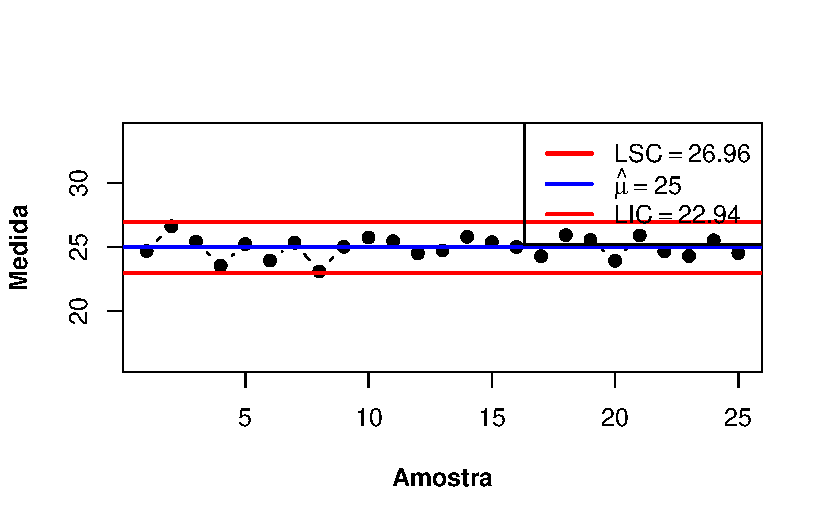
\includegraphics[keepaspectratio]{C2_PlotOfVariables_files/figure-pdf/EX_R_BASE_1-1.pdf}}

\subsection{\texorpdfstring{R usando
\texttt{ggplot2}}{R usando ggplot2}}

\pandocbounded{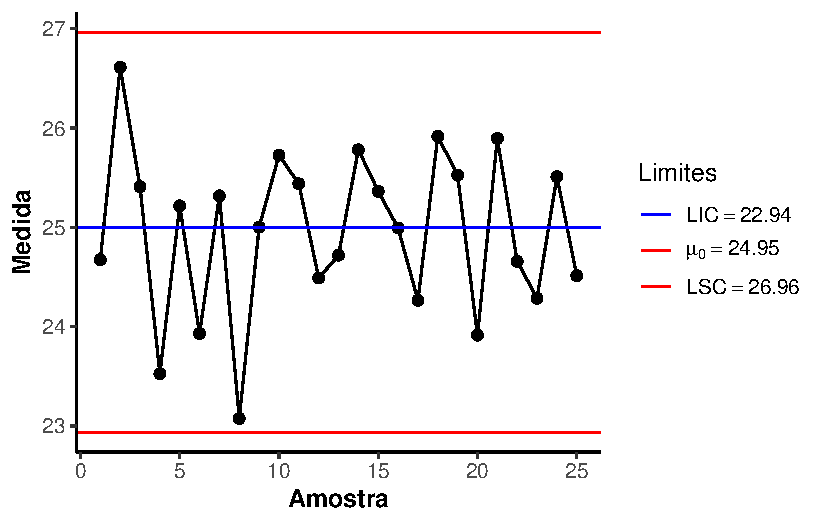
\includegraphics[keepaspectratio]{C2_PlotOfVariables_files/figure-pdf/EX_R_ggplot2_1-1.pdf}}

\subsection{Python}

\begin{verbatim}
(18.0, 32.0)
\end{verbatim}

\pandocbounded{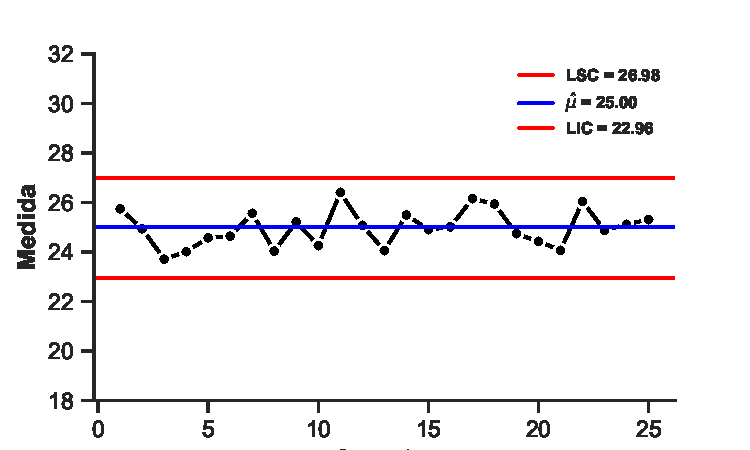
\includegraphics[keepaspectratio]{C2_PlotOfVariables_files/figure-pdf/EX_PYTHON_1-1.pdf}}

\subsection{\texorpdfstring{Demais Variações do Gráfico de Controle de
\(\bar{X}\)}{Demais Variações do Gráfico de Controle de \textbackslash bar\{X\}}}\label{demais-variauxe7uxf5es-do-gruxe1fico-de-controle-de-barx}

\subsubsection{\texorpdfstring{Gráficos de Médias e Amplitudes
(\(\bar{X}\) e
\(R\))}{Gráficos de Médias e Amplitudes (\textbackslash bar\{X\} e R)}}\label{gruxe1ficos-de-muxe9dias-e-amplitudes-barx-e-r}

Na prática da construção de gráficos de controle, a média (\(\mu\)) e o
desvio-padrão (\(\sigma\)) do processo raramente são conhecidos.
Portanto, esses parâmetros precisam ser estimados a partir de dados
amostrais. A premissa fundamental é que essas amostras, ou subgrupos,
sejam coletadas em um momento em que o processo esteja operando sob
controle estatístico.

Para isso, Walter Shewhart sugeriu um método prático: a coleta de
\textbf{\(m\)} subgrupos (geralmente entre 20 a 25) de tamanho
\textbf{\(n\)} relativamente pequeno (4, 5 ou 6 itens cada). Essa
abordagem visa a construção de ``subgrupos racionais'' com um baixo
custo de amostragem.

Para estimar a média global do processo, \(\mu\), utilizamos a média das
médias de todos os subgrupos. Sejam
\(\bar{X}_1, \bar{X}_2, \ldots, \bar{X}_m\) as médias de cada um dos
\textbf{\(m\)} subgrupos. O melhor estimador para \(\mu\) é a grande
média, denotada por \(\bar{\bar{X}}\):
\[\bar{\bar{X}} = \frac{\sum_{i=1}^{m} \bar{X}_i}{m}.\]

Onde \(\bar{X}_i\) é a média amostral do i-ésimo subgrupo. Por essa
razão, o valor de \(\bar{\bar{x}}\) será usado como a \textbf{linha
central (LC)} do gráfico \(\bar{X}\).

Para construir os limites de controle, tanto do gráfico \(\bar{X}\)
quanto do gráfico R, precisamos de um estimador para o desvio-padrão do
processo, \(\sigma\). Essa estimativa pode ser obtida a partir dos
desvios-padrões de cada subgrupo ou, mais comumente, a partir das
\textbf{amplitudes} das amostras. Para esta análise, optaremos pelo
método das amplitudes.

A amplitude (\(R\)) de uma amostra é a diferença entre o valor máximo e
o valor mínimo observados nela: \[R = X_{\text{max}} - X_{\text{min}}\]

Sendo \(R_1, R_2, \ldots, R_m\) as amplitudes de cada um dos
\textbf{\(m\)} subgrupos, calculamos a amplitude média (\(\bar{R}\))
como: \[\bar{R} = \frac{\sum_{i=1}^{m} R_i}{m}\]

\subsubsection{Construção do Gráfico
R}\label{construuxe7uxe3o-do-gruxe1fico-r}

O Gráfico R monitora a variabilidade do processo ao longo do tempo. Sua
linha central é a amplitude média (\(\bar{R}\)), e seus limites de
controle são calculados usando constantes estatísticas que dependem do
tamanho do subgrupo (\(n\)).

\begin{itemize}
\tightlist
\item
  \textbf{LSC} = \(D_4 \bar{R}\)
\item
  \textbf{LM} = \(\bar{R}\)
\item
  \textbf{LIC} = \(D_3 \bar{R}\)
\end{itemize}

É importante lembrar que a amplitude média também nos fornece um
estimador não viesado para o desvio-padrão do processo, \(\sigma\),
através da seguinte relação: \[\hat{\sigma} = \frac{\bar{R}}{d_2}\]

\subsubsection{\texorpdfstring{Construção do Gráfico
\(\bar{X}\)}{Construção do Gráfico \textbackslash bar\{X\}}}\label{construuxe7uxe3o-do-gruxe1fico-barx}

Com as estimativas da média (\(\bar{\bar{x}}\)) e da variabilidade (via
\(\bar{R}\)) do processo, podemos construir os limites de controle para
o gráfico \(\bar{X}\), que monitora a tendência central do processo.

\begin{equation}\phantomsection\label{eq-DEF_LIMITS_R_CHARTS}{
\text{Limites} = \begin{cases} \bar{\bar{X}} + A_2 \bar{R}, \quad \text{se o Limite for Inferior} \\ \bar{\bar{X}}, \quad \text{se o Limite for Central} \\ \bar{\bar{X}} - A_2 \bar{R}, \quad \text{se o Limite for Superior} \end{cases}.
}\end{equation}

As constantes \(A_2, d_2, D_3\) e \(D_4\) são tabeladas e dependem do
tamanho do subgrupo (\(n\)). Elas podem ser encontradas em apêndices de
livros de referência sobre o tema, como o ``Introdução ao Controle de
Qualidade'' de Montgomery.

\subsubsection{\texorpdfstring{Gráficos de Médias e Desvio Padrão
(\(\bar{X}\) e
\(R\))}{Gráficos de Médias e Desvio Padrão (\textbackslash bar\{X\} e R)}}\label{gruxe1ficos-de-muxe9dias-e-desvio-padruxe3o-barx-e-r}

\section{\texorpdfstring{Gráfico de Controle para
\(R\)}{Gráfico de Controle para R}}\label{gruxe1fico-de-controle-para-r}

\section{\texorpdfstring{Gráfico de Controle para
\(S\)}{Gráfico de Controle para S}}\label{gruxe1fico-de-controle-para-s}

\bookmarksetup{startatroot}

\chapter{Curva Característica da Operação e Compimento Médio da
Sequência}\label{curva-caracteruxedstica-da-operauxe7uxe3o-e-compimento-muxe9dio-da-sequuxeancia}

\section{Introdução}\label{introduuxe7uxe3o-1}

\section{Curva Característica da Operação
(CCO)}\label{curva-caracteruxedstica-da-operauxe7uxe3o-cco}

\section{Compimento Médio da Sequência
(CMS)}\label{compimento-muxe9dio-da-sequuxeancia-cms}

\bookmarksetup{startatroot}

\chapter{Gráficos de Controle para
Atributos}\label{gruxe1ficos-de-controle-para-atributos}

\bookmarksetup{startatroot}

\chapter{Índice de Capacidade}\label{uxedndice-de-capacidade}

\bookmarksetup{startatroot}

\chapter*{Referências}\label{referuxeancias}
\addcontentsline{toc}{chapter}{Referências}

\markboth{Referências}{Referências}

\phantomsection\label{refs}




\end{document}
